\documentclass{article}

% Packages
\usepackage{booktabs}
\usepackage{multirow} 
\usepackage{multicol} 
\usepackage{fullpage} 
\usepackage{fancyhdr} 

\usepackage[headsep=1cm,total={6.5in, 8.5in},margin=1in]{geometry}

\usepackage{cancel}
\usepackage{amsmath,amssymb, amsthm, amsfonts}
\usepackage[fleqn]{nccmath}
\usepackage{gensymb}% useless
\usepackage{listings}
\usepackage{color}\usepackage{multirow}
\usepackage{siunitx}

\usepackage[%  
    colorlinks=false,
    linkcolor=red
]{hyperref}

\usepackage[fleqn]{nccmath} % for left aligning equations
\usepackage[T1]{fontenc}
\usepackage[utf8]{inputenc}
\usepackage{alphabeta}
\usepackage[english, greek]{babel}
\usepackage{graphicx}
\usepackage{pgfplots}
\usepackage{tabularx}
\usepackage{pdfpages}

\makeatletter
\renewcommand\verbatim@font{\normalfont\fontencoding{T1}\ttfamily}
\makeatother

\lstset{frame=tb,
  aboveskip=3mm,
  belowskip=3mm,
  showstringspaces=false,
  columns=flexible,
  basicstyle={\small\ttfamily},
  numbers=none,
  numberstyle=\tiny\color{gray},
  keywordstyle=\color{blue},
  commentstyle=\color{dkgreen},
  stringstyle=\color{mauve},
  breaklines=true,
  breakatwhitespace=true,
  tabsize=3
}

% Header Commands
\newcommand{\settitle}	{EE119C Project}
\newcommand{\names} {Christian Miranda}

% User defined commands
\newcommand{\RR}{\mathbb{R}} % typing \RR prints the Blackboard R used for Real Numbers
\newcommand{\NN}{\mathbb{N}} % typing \NN prints the Blackboard N used for Natural Numbers
\newcommand{\ZZ}{\mathbb{Z}} 
\newcommand{\GCD}{\textrm{GCD}}
\newcommand{\Expectation}[1]{\mathbb{E}[#1]}
\newcommand{\Var}[1]{\mathr2m{2Var[#1]}}
\newcommand{\Cov}[1]{\mathrm{Cov[#1]}}
\newcommand{\Cancel}[2][black]{{\color{#1}\cancel{\color{black}#2}}}

% Document start
\begin{document}
\selectlanguage{English}

% Don't draw header on first page 
\thispagestyle{empty} 

% Header to draw on each page but the first
\pagestyle{fancy}\lhead{\names} \chead{\settitle} \rhead{\today}

% Page 1
\begin{titlepage}
    \begin{center}
        \vspace*{1cm}

        \Large
        \textbf{Single Chip TB-303}

        \vspace{0.5cm}
            Spring 2025

        \vspace{1.5cm}

        \textbf{Christian Miranda}

        \vfill

        % Last revised June 11, 2024

        \vspace{0.8cm}

        California Institute of Technology \\
        Department of Electrical Engineering \\
        Pasadena, California \\
        EE119C 
         
    \end{center}
\end{titlepage}

\newpage

    \section*{Introduction}

    TODO.

    \section*{Theory of Operation}

    TODO.

    \section*{NEC $\mu$COM-43 Clone}

    TODO.

    \section*{NCO}

        A simple NCO has the following block diagram:
        
        \medskip

        \begin{figure}[!ht]
            \centering
            \includegraphics[width=\textwidth]{noc_bd_1.png}
            \caption{NCO Block Diagram}
            \label{fig:fig1}
        \end{figure}

        The accumulated phase is

        \begin{gather}
            % Accumulated phase equation.
            \phi_1[n] = \phi_1[n-1] + 2 \pi f_i [n], \; \; \;
            \phi[n] = \phi_1[n] + \theta_i[n]
        \end{gather}

        Where $\phi_1[n]$, $\phi[n]$, $\theta_1[n]$ are real numbers and n
        is a non-negative integer. Here, $\phi_1[n]$ represents the accumulated
        phase, while $\phi[n]$ represents the accumulated phase plus an 
        instantaneous phase offset, $\theta_i[n]$, that is used to phase-shift
        the output wave without accumulating this phase shift.

        % This is stupid.
        \vspace{3mm}
        
        A digital output waveform can be generated by using a look-up table 
        (LUT) of pre-calculated values that correspond to a function (often a
        sinusoid). For this example, we will use cosine.

        % This is stupid.
        \vspace{3mm}

        We first take $\phi[n] \bmod 2\pi$ so that our phase is within 
        $[0, 2\pi)$. Our table will have $N$ entries of values corresponding to
        $y_k = cos(\frac{2\pi k}{N})$, where $k \in [0, N]$. Since we want
        $cos(\phi[n]) \approx cos(\frac{2\pi k}{N})$, we see that solving 
        $\phi [n] = \frac{2 \pi k}{N}$ gives us our index, 
        $k = \text{round}(\frac{\phi [n] N}{2 \pi})$. 

        % This is stupid.
        \vspace{3mm}

        \newpage

        We can scale (1) by $\frac{N}{2 \pi}$ so that we may use
        the phase accumulator directly to index the LUT. This gives us

        \begin{gather}
            \frac{N}{2 \pi} \phi_1[n] = \frac{N}{2 \pi} \phi_1[n - 1] + N f_i[n], \quad
            \frac{N}{2 \pi} \phi[n] = \frac{N}{2 \pi} \phi_1[n] + \frac{N}{2 \pi} \theta_i[n]
            \\
            k_1[n] = k_1[n - 1] + N f_i[n], \quad k[n] = k_1[n] + \frac{N}{2 \pi} \theta_i[n]
        \end{gather}
        
        Where $k_1[n]$ is the index corresponding to the cosine of the 
        accumulated phase and $k[n]$ is the index corresponding to the accumulated
        phase plus an instantaneous phase offset. Note that both $k_1[n]$ and
        $k[n]$ both need to be taken modulo $N$, since there are only $N$ 
        entries in the LUT.

        \begin{gather}
            k_1[n] = (k_1[n - 1] + N f_i[n]) \bmod N, \quad 
            k[n] = (k_1[n] + \frac{N}{2 \pi} \theta_i[n]) \bmod N
        \end{gather}
            
        We can avoid doing modulo by making the table size equal to the number
        of bits in the phase accumulator, such that unsigned addition overflow
        will wrap to zero, thus giving us modulo N "for free".

        \vspace{3mm}

        Our practical design will thus look as follows:
        
        \begin{figure}[!ht]
            \centering
            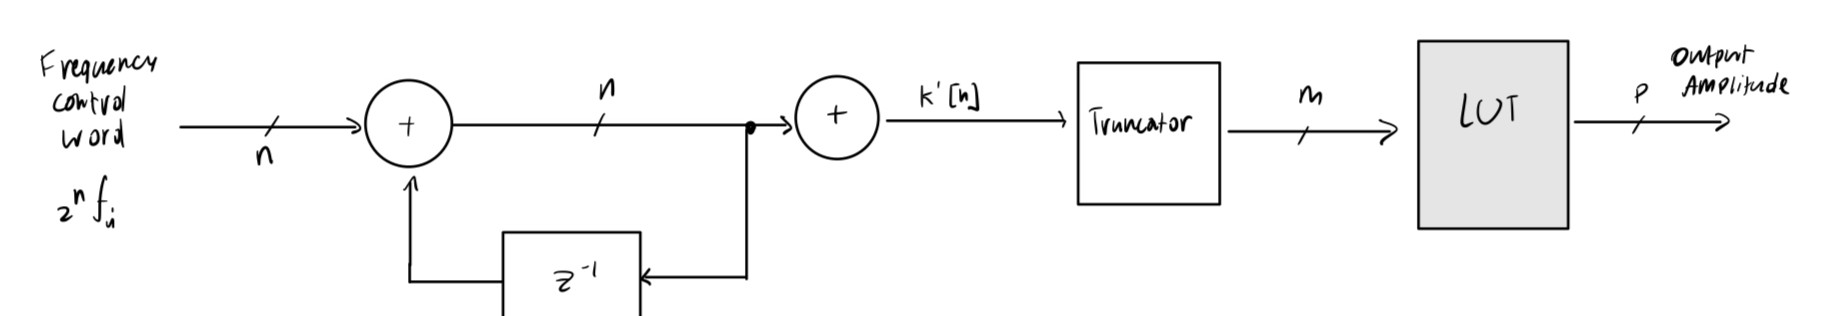
\includegraphics[width=\textwidth]{nco_bd_2.png}
            \caption{Practical NCO Block Diagram}
            \label{fig:fig2}
        \end{figure}
        
        The hardware implementation will be as follows:


        \begin{figure}[!ht]
            \centering
            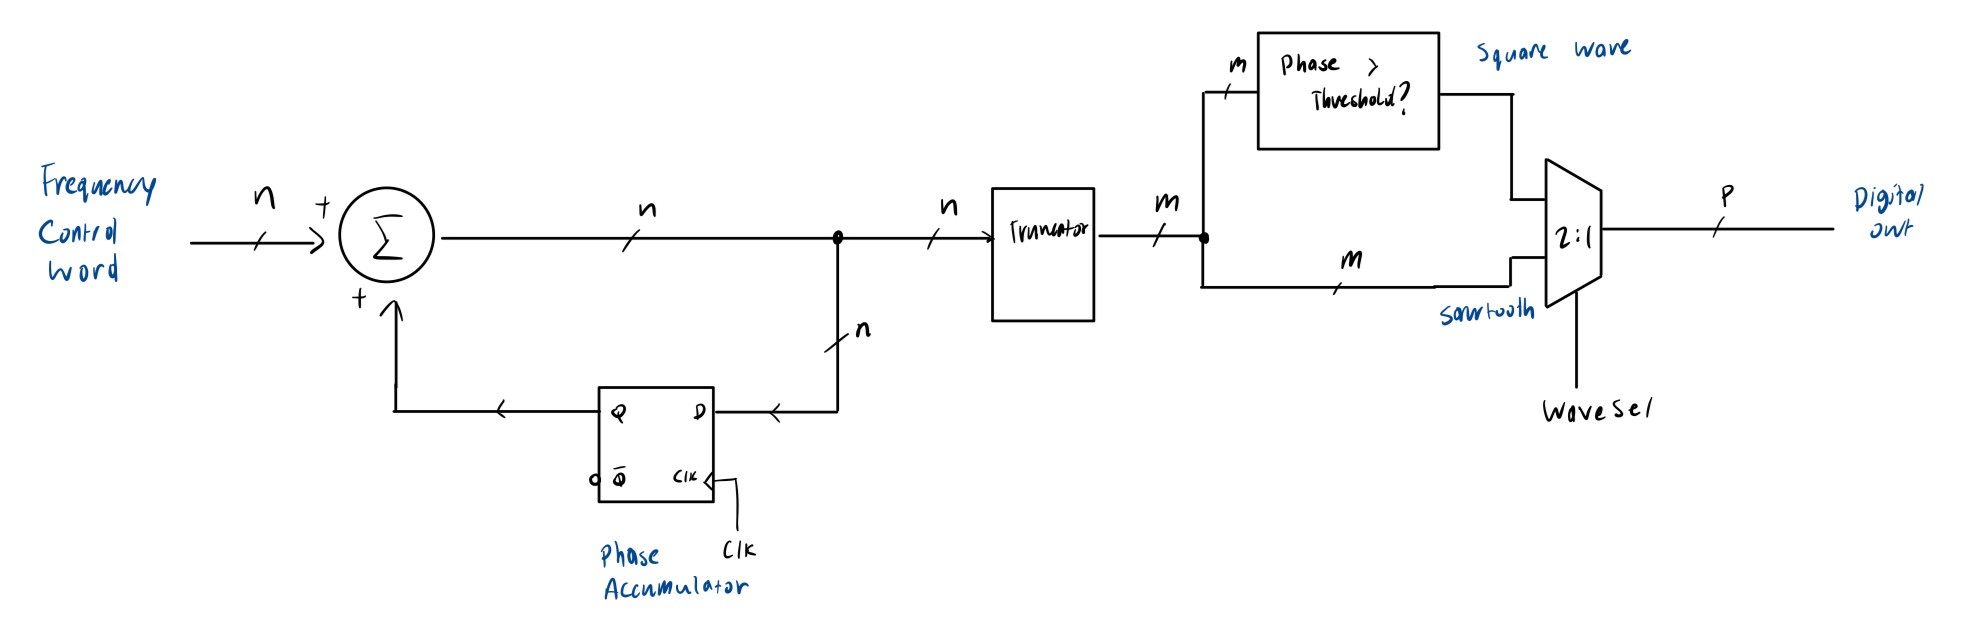
\includegraphics[width=\textwidth]{nco_bd_3.png}
            \caption{Hardware NCO Block Diagram}
            \label{fig:fig3}
        \end{figure}

        Our maximum frequency is determined by our sample rate according to
        Nyquist–Shannon sampling theorem. 

        % This is stupid.
        \vspace{3mm}
        

    \section*{Digital Ladder Filter}

    \section*{Numerically Controlled Amplifier}

    \section*{Testing in Simulation:}
    
    \section*{Testing in Hardware:}

\end{document}